\documentclass[air,article,submit,moreauthors]{Definitions/mdpi}

\firstpage{1}
\makeatletter
\setcounter{page}{\@firstpage}
\makeatother
\pubvolume{1}
\issuenum{1}
\articlenumber{0}
\pubyear{2026}
\copyrightyear{2026}
\datereceived{ }
\daterevised{ }
\dateaccepted{ }
\datepublished{ }

\Title{WRF Cold-Pool Sensitivities Relevant to Winter-Ozone Modelling in the Uinta Basin}

\newcommand{\orcidauthorA}{0000-0003-0305-4090}
\newcommand{\orcidauthorB}{0009-0009-9083-6568}
\Author{John R. Lawson $^{1,2,}$*\orcidA{}, Michael J. Davies $^{1}$\orcidB{}, Loknath Dhar $^{1,3}$ and Seth N. Lyman $^{1,3}$}
\AuthorNames{John R. Lawson, Michael J. Davies, Loknath Dhar and Seth N. Lyman}

\address{%
$^{1}$ \quad Bingham Research Center, Utah State University, Vernal, UT 84078, USA;\\
$^{2}$ \quad Department of Mathematics and Statistics, Utah State University, Logan, UT 84322, USA;\\
$^{3}$ \quad Department of Chemistry and Biochemistry, Utah State University, Logan, UT 84322, USA}
\corres{Correspondence: john.lawson@usu.edu}

\abstract{Cold-pool structure controls the confinement and transport environment relevant to surface wintertime ozone in the mountainous Uinta Basin, Utah, USA, but point surface values alone do not establish that structure.
We evaluated deterministic responses in Weather Research and Forecasting (WRF) simulations of the 2 February 2013 episode to the supplied Global Forecast System (GFS) or North American Model (NAM) driving analysis, nest feedback, boundary-layer and surface-layer treatment, slope-aware radiation, and static-terrain source.
Across a common five-hour sample, GFS-driven members were warmer at the evaluated surface sites, approximately 3.6\,K less stable through 50--500\,m above ground level, and 0.8--1.0\,m\,s$^{-1}$ faster in fixed-layer transport wind than feedback-matched NAM members.
GFS-driven members also retained a smaller footprint-mean, vertically integrated heat deficit under all seven definitions, although every simulation gained heat deficit over the retained window.
The repeated separation is therefore a driving-product state response rather than demonstrated faster cold-pool loss.
Controlled feedback and physics responses were smaller and metric dependent, while bounded terrain and fine-grid process diagnostics showed spatial structure that the station sample could miss without establishing terrain superiority, resolution benefit, basin export, or inversion depth.
The study provides a meteorological result with implications for subsequent air-chemistry modelling; it does not contain a chemistry calculation or identify the initial-versus-lateral-boundary contribution to the driving-product response.}

\keyword{ozone; WRF; meteorology; modelling; cold-air pool; complex terrain; model resolution}

\begin{document}

\section{Introduction}
\label{sec:v3-introduction}

Surface wintertime ozone in the Uinta Basin develops within a snow-covered, persistently stable boundary layer in which weak mixing and transport can confine precursors near the surface \citep{Ahmadov2015-zm,Neemann2015-ws,Davies2025-wy}.
For a coupled weather--chemistry calculation, the relevant meteorological information therefore extends beyond 2\,m temperature error to the simulated depth, stability, heat storage, and transport of the lower atmosphere.
Point observations remain indispensable, but a horizontally separated surface network does not by itself validate inversion depth or the three-dimensional mixing volume supplied to chemistry.

Meteorological, emissions, photolysis, deposition, and chemical-mechanism errors can compensate for one another in coupled simulations.
For example, holding meteorology fixed while changing emissions can alter ozone agreement without identifying a unique inventory error \citep{Ahmadov2015-zm}.
Cumulative changes in emissions, leaf area, deposition, and meteorology likewise complicate attribution, and improved modelled temperature profiles need not translate directly into improved ozone profiles \citep{Matichuk2017-bq}.
Credible meteorology is thus a prerequisite for chemical attribution rather than proof that meteorology is the dominant or only uncertainty.

Previous WRF studies also show why the experimental design must remain explicit.
Bundled snow, microphysics, and grid choices can produce large case-specific responses, while evaluation and chemistry grids need not sample the same structure \citep{Neemann2015-ws}.
Four-dimensional data-assimilation responses can depend on the nudged variables, input data, and scheme-dependent boundary-layer diagnosis \citep{Tran2018-ax}.
The present study therefore treats controlled contrasts, failed tests, and within-run diagnostics as distinct kinds of evidence.

Following preliminary experiments and review of the archived simulation family, we ask:

\begin{enumerate}
  \item Does the lower-layer response to the supplied GFS or NAM driving analysis recur under both one-way and two-way nest feedback?
  \item How large are the controlled nest-feedback, boundary-layer and surface-layer, and slope-aware-radiation responses relative to the driving-product response on common diagnostics?
  \item What reproducible atmospheric response appears across controlled static-terrain-source brackets on the same WRF grid, and which interpretations remain unsupported?
  \item What do surface, common-height, and footprint heat-deficit diagnostics reveal together that any single station metric can miss?
\end{enumerate}

Terrain-source contrasts require area-weighted geometry diagnostics because a station-only summary can miss a rim- or slope-confined response.
The archived simulations use the compact X0--X10 identifiers, which link configurations in the text and tables to the run inventory.
The present paper evaluates the meteorological state that a later chemistry calculation would receive; it contains no chemistry calculation and makes no ozone prediction.

\section{Materials and Methods}
\label{sec:v3-methods}

\subsection{Case, Observations, and Evaluation Domains}
\label{sec:v3-case}

The case is 2 February 2013 within a broader January--February period of snow cover, cold-pool conditions, and elevated ozone in the Uinta Basin \citep{Neemann2015-ws,Ahmadov2015-zm,Tran2018-ax}.
The WRF integrations cover 1200--1800 Coordinated Universal Time (UTC), corresponding to 0500--1100 Mountain Standard Time (MST; UTC$-7$).
The retained analysis window covers 1400--1800 UTC, or 0700--1100 MST, and excludes both the 1200 UTC initialised output and the 1300 UTC first-hour forecast.
This leaves five hourly samples for every common-window contrast.
Surface observations were obtained through the Synoptic Data PBC Mesonet API for 2\,m temperature at 11 sites, 10\,m wind speed at 10 sites, and surface pressure at 9 sites.\footnote{Synoptic Data PBC Mesonet API Time Series service: \url{https://docs.synopticdata.com/services/time-series}.}
Subhourly reports were mean-averaged within each UTC clock hour.
The stations span basin-floor, sidewall, and bench locations but are neither spatially uniform nor area weighted; as the focus herein is not verification against observations, we leave further evaluation to future studies.
The 1\,km d02 domain was selected for the common observation comparisons because seven stations fall outside the usable d03 interior, leaving four usable d03 station columns.
Figure~\ref{fig:v3-locator} combines the reporting-station geometry with the full nested-domain layout.
Use of d02 does not establish that d02 and d03 produce the same response, and a common-support transfer test remains future work.
Four stations spanning the basin floor and benches provide surface context from 31 January 0000 UTC to 4 February 0000 UTC.
Observed and modelled surface potential temperature for a two-site structural index was calculated as $\theta=T(1000/p)^{0.2854}$, with $T$ in kelvin and $p$ in hPa.
The index is Mountain Home on the north-west bench minus Pariette Draw on the basin floor, with both locations labelled in Figure~\ref{fig:v3-locator}.
Their horizontal separation requires treating the index as a surface contrast rather than free-air inversion strength or cold-pool depth.

Episode-scale ozone context came from the US Environmental Protection Agency (EPA) Air Quality System (AQS) AirData daily archive for 1 January--28 February 2013.
We retained the EPA-reported ``Ozone 8-hour 2015'' daily-summary row at Ouray, Redwash, Roosevelt, Vernal, and Little Mountain. 
All five sites contained one daily row on each of the 59 local calendar dates; within-day observation coverage ranged from 47\% to 100\% and is marked explicitly in the figure.
The satellite panel in Figure~\ref{fig:v3-episode-context} uses the National Aeronautics and Space Administration (NASA) Global Imagery Browse Services (GIBS) Terra Moderate Resolution Imaging Spectroradiometer (MODIS) corrected-reflectance 7-2-1 layer for 2 February 2013.\footnote{NASA Worldview and GIBS: \url{https://worldview.earthdata.nasa.gov/}.}

\begin{figure}[H]
\centering
\begin{minipage}[t]{0.49\textwidth}
\centering
\textbf{(a)}\\[-2pt]
\IfFileExists{figures/wrf_geographic_locator_d01_d03.pdf}{%
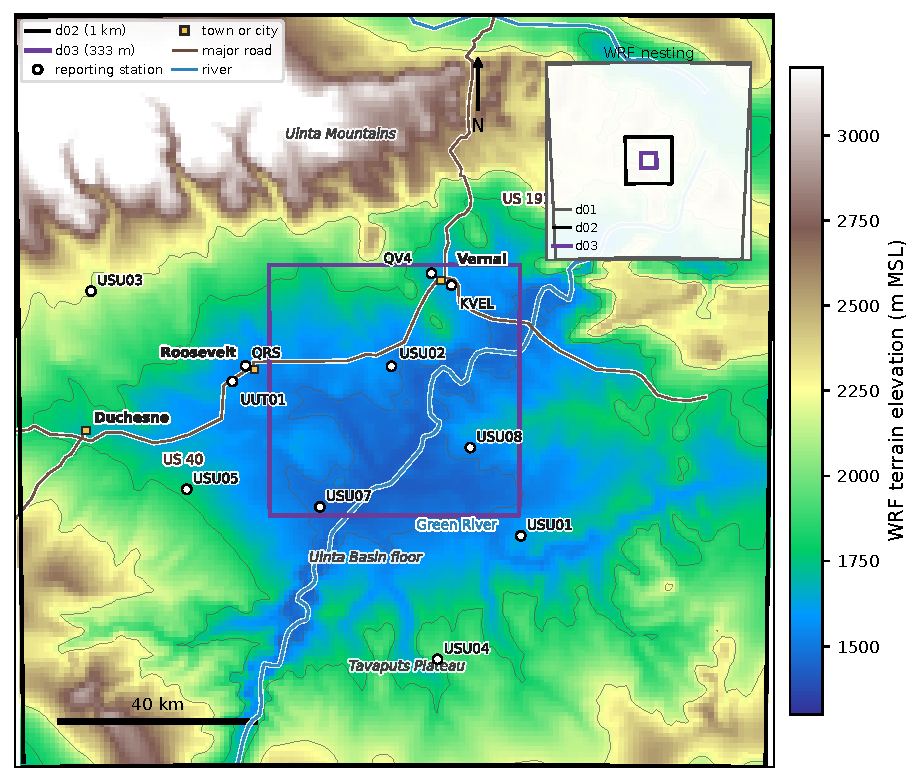
\includegraphics[width=\linewidth]{figures/wrf_geographic_locator_d01_d03.pdf}%
}{\fbox{\parbox[c][0.42\textheight][c]{0.90\linewidth}{\centering Geographic locator unavailable.}}}
\end{minipage}\hfill
\begin{minipage}[t]{0.49\textwidth}
\centering
\textbf{(b)}\\[-2pt]
\IfFileExists{verification/figures/candidates/wrf_nested_domains_d01_d03.png}{%
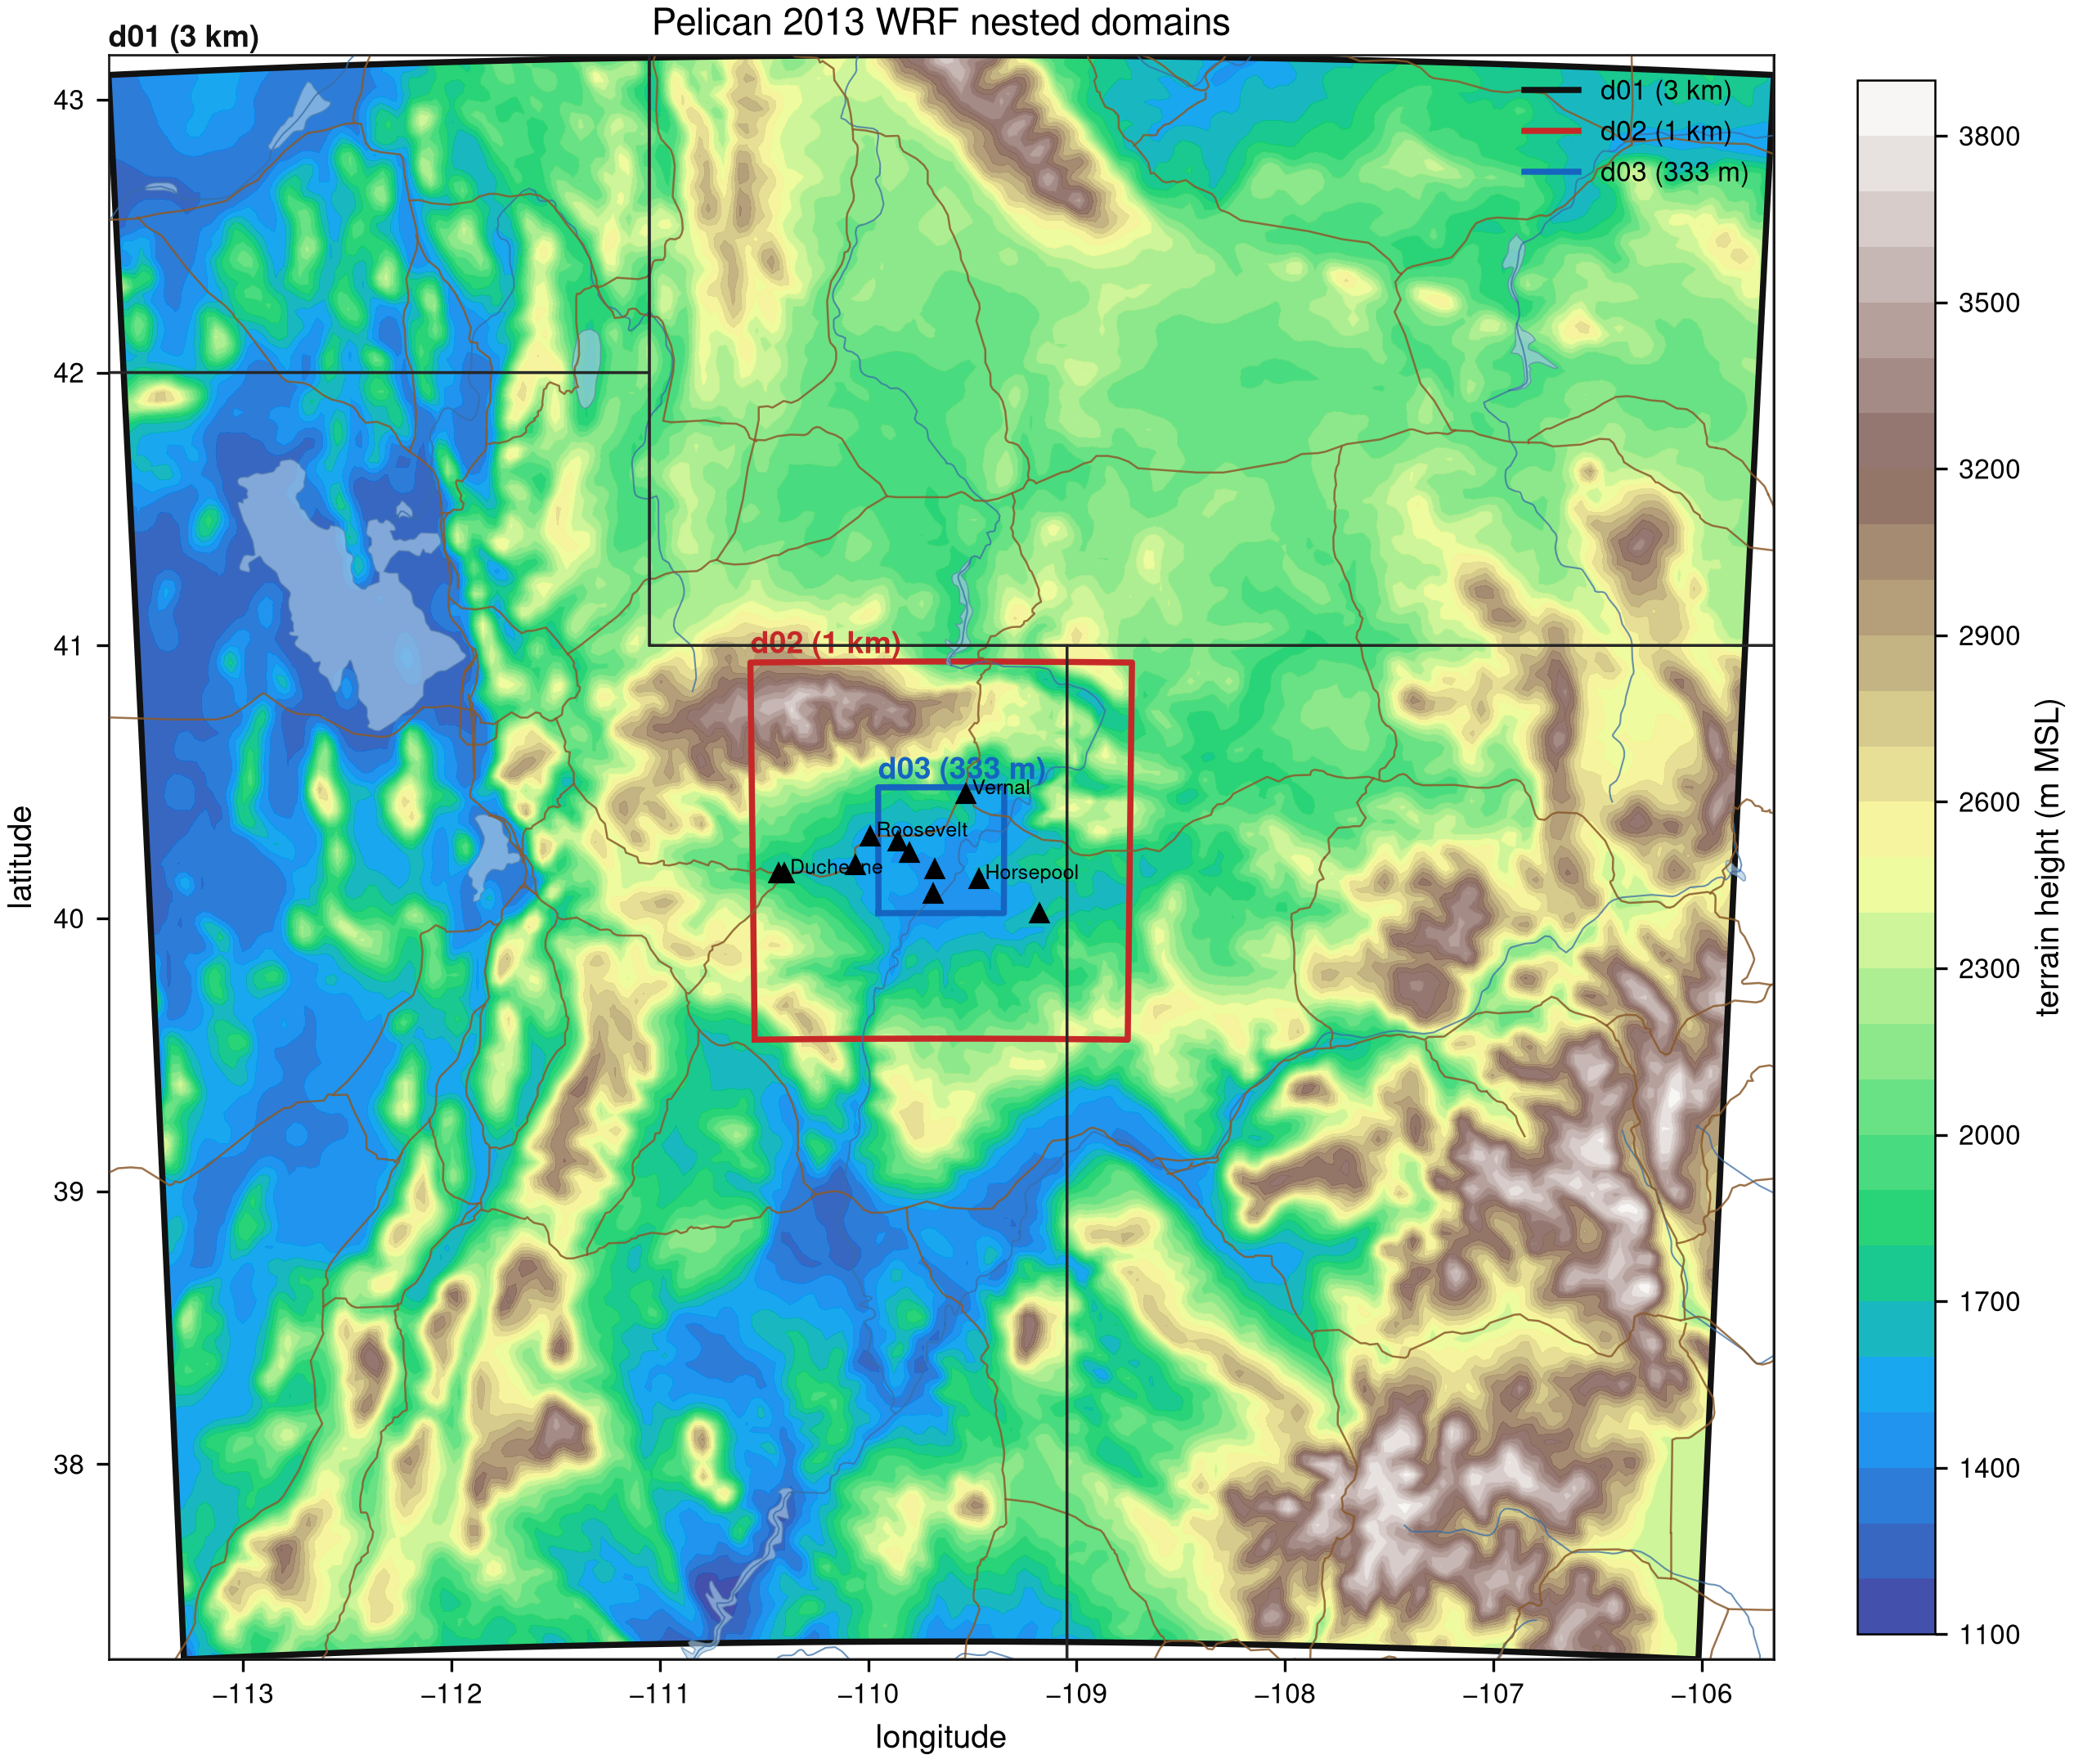
\includegraphics[width=\linewidth]{verification/figures/candidates/wrf_nested_domains_d01_d03.png}%
}{\fbox{\parbox[c][0.42\textheight][c]{0.90\linewidth}{\centering Three-domain WRF grid layout unavailable.}}}
\end{minipage}
\caption{Geographic and sampling orientation for the evaluation.
(a) The d02 terrain, reporting stations, and d03 interior define the common evaluation setting.
(b) The d01--d02--d03 WRF grid layout places that setting within the full three-domain configuration.
Seven of the eleven reporting stations fall outside the usable d03 interior, which is why d02 supplies the full-network sample; neither panel constitutes a resolution evaluation.}
\label{fig:v3-locator}
\end{figure}

\subsection{WRF Configuration and Archived Simulation Family}
\label{sec:v3-family}

The controlled six-hour simulations used WRF version 4.8.0, initialised at 1200 UTC with either Global Forecast System (GFS) or North American Model (NAM) analyses and supplied with source-specific lateral boundary conditions through 1800 UTC on 2 February 2013.
These are retrospective simulations driven by analyses rather than six-hour operational forecasts.
The design does not separate the initialised state from the subsequent lateral-boundary contribution.
We used three nested computational domains, d01--d03, with horizontal grid spacings of 3\,km, 1\,km, and 333.333\,m.
The controlled family used 75 eta levels concentrated near the surface, with approximately 20\,m separation among the lowest mass levels, and a 50\,hPa model top.
The Advanced Research WRF Model Version 4 is cited following Skamarock et al. (2019, NCAR/TN-556+STR).\footnote{\url{https://doi.org/10.5065/1dfh-6p97}}
The reference physics suite used Thompson microphysics, Rapid Radiative Transfer Model for General Circulation Models (RRTMG) longwave and shortwave radiation, the revised fifth-generation Pennsylvania State University--National Center for Atmospheric Research Mesoscale Model (MM5) similarity surface layer, the Noah land-surface model, and the Yonsei University (YSU) planetary boundary layer (PBL) scheme.\footnote{The WRF physics-reference register identifies Thompson et al. (2008), Iacono et al. (2008), Jim\'enez et al. (2012), Tewari et al. (2004), and Hong et al. (2006) for these options: \url{https://www2.mmm.ucar.edu/wrf/users/physics/phys_references.html}.}
Grid and observation four-dimensional data assimilation were disabled.
Departures from that reference configuration are listed by simulation in Table~\ref{tab:v3-family}.

Static terrain entered through the WRF Preprocessing System and was held fixed within each controlled pair.
The custom fine source used 3-arc-second terrain, the default source was 30-arc-second class, and the deliberately coarse source used the 5-arc-minute GMTED2010 product.
At approximately $40^{\circ}$N their nominal north--south spacings are about 90\,m, 900\,m, and 9\,km, respectively, and these static-source spacings are distinct from WRF horizontal grid spacing.
Land-surface initial fields, including snow, entered through the source-specific meteorological preprocessing, so the GFS--NAM treatment does not isolate a snow-field contribution.
Our experiment configurations split into four scientific branches: driving-data product, boundary-layer and radiation treatments, nest feedback, and static-terrain source.
The X7 and X8 configurations differ from the controlled family in several dimensions at once and enter only as design context (Section~\ref{sec:v3-resolution}) --- again, interpretation must be careful when changes in output may result from confounding effects.

\begin{table}[H]
\caption{The archived simulation family.
Every run uses WRF 4.8.0, three nests at 3/1/0.333\,km with 75 levels, Thompson microphysics, RRTMG radiation, and Noah land surface unless stated.
``Fine terrain'' is the custom 3-arc-second source, ``default terrain'' is 30-arc-second class, and ``coarse terrain'' is the 5-arc-minute GMTED2010 source; static-source spacing is not model-grid spacing.}
\label{tab:v3-family}
\centering
\small
\begin{tabularx}{\textwidth}{llL}
\toprule
Code & Product, feedback & Configuration and role \\
\midrule
X0  & NAM, one-way & fine-terrain YSU/MM5 control for X1, X3, X4, and X9 \\
X1  & NAM, one-way & X0 plus slope radiation and shading \\
X2  & NAM, one-way & X1 with MYJ/Eta instead of YSU/MM5 \\
X3  & NAM, one-way & default-terrain reference configuration \\
X4  & NAM, one-way & deliberately coarse 5-arc-minute terrain \\
X5  & NAM, two-way & default terrain \\
X6  & GFS, two-way & default terrain \\
X7  & NAM, two-way & 1 km inner grid and 24 h integration; design context only \\
X8  & NAM, one-way & four domains to 111 m and 50 levels; design context only \\
X9  & NAM, two-way & X0 with two-way feedback \\
X10 & GFS, one-way & default terrain \\
\bottomrule
\end{tabularx}
\end{table}

\subsection{Controlled Contrasts and Estimands}
\label{sec:v3-contrasts}

We contrast simulations, identifying the dominant lever on the simulation's sensitivity, and its magnitude (Table~\ref{tab:v3-comparisons}).  The table is ordered by scientific role.
The four default-terrain simulations X3, X5, X6, and X10 form a fundamental two-by-two matrix that buttresses our analyses. 
Native GFS and NAM data provides 27 and 40 metgrid levels, respectively.

(The remaining controlled contrasts enter on their own design and evidence: the X2-minus-X1 scheme treatment, X1-minus-X0 slope-radiation treatment, X9-minus-X0 fine-terrain feedback treatment, and the pairwise X3/X0/X4 terrain-source brackets.)

\begin{table}[H]
\caption{Controlled contrasts referenced in this study, their differencing orientation, and their scientific use.}
\label{tab:v3-comparisons}
\centering
\small
\begin{tabularx}{\textwidth}{lLL}
\toprule
Operation & Isolated lever & Use in this study \\
\midrule
X6 $-$ X5 & driving product (two-way) & primary controlled contrast \\
X10 $-$ X3 & driving product (one-way) & primary controlled contrast \\
X2 $-$ X1 & PBL and surface-layer scheme & secondary controlled contrast \\
X1 $-$ X0 & slope radiation and shading & spatial diagnostic with an archive limitation \\
X3 $-$ X5 & feedback, NAM, default terrain & secondary robustness contrast \\
X10 $-$ X6 & feedback, GFS, default terrain & secondary robustness contrast \\
X9 $-$ X0 & feedback, NAM, fine terrain & secondary robustness contrast \\
(X10$-$X6)$-$(X3$-$X5) & driving-product-by-feedback interaction & secondary interaction contrast \\
X3 $-$ X0 & terrain source, default vs fine & bounded terrain response; no source ranking \\
X3 $-$ X4 & terrain source, default vs coarse & bounded terrain response; no source ranking \\
X0 $-$ X4 & terrain source, fine vs coarse & bounded terrain response; no source ranking \\
\bottomrule
\end{tabularx}
\end{table}

\subsection{Design Exclusions: Resolution and Legacy Context}
\label{sec:v3-resolution}

X7, X0, and X8 do not form a controlled resolution sequence because their integrations differ in forecast age, domain geometry, feedback, vertical levels, terrain placement, radiation settings, and output cadence.
They are retained only to document the exclusion; no X8 diagnostic is reported in this paper.

\subsection{Surface and Common-AGL Diagnostics}
\label{sec:v3-common-agl}

Modelled 2\,m dry-bulb temperature, 10\,m wind, and surface pressure were sampled at the nearest d02 cell to each station.
None of the selected cells lay on steep terrain or an obviously unrepresentative model location.
Across the eleven fixed columns, model terrain offset from reported station elevation spanned -32\,m to 14\,m.
While this justifies the nearest-neighbour approach, the pairing of WRF output to observation value does not remove (wind, solar) exposure, slope angle, land-cover use, or network-coverage deficiency.
Mass-level height above ground level (AGL) was calculated from perturbation plus base geopotential relative to local WRF terrain height.
Grid-relative winds were destaggered and rotated to earth-relative components.
Model-level potential temperature $\theta$ and horizontal wind components were interpolated linearly at 25\,m increments from 50 to 500\,m AGL at each station column.
Fixed-layer stability was defined as

\begin{equation}
S_{50:500}=\theta(500\,\mathrm{m})-\theta(50\,\mathrm{m})
\end{equation}

The transport-wind proxy was defined as

\begin{equation}
U_{50:500}=\left(\bar{u}^{2}+\bar{v}^{2}\right)^{1/2}.
\end{equation}

where the bars denote height means from 50 to 500 m AGL.
This wind-derived quantity is a fixed-layer transport proxy and does not sample flow through a basin boundary, pollutant residence time, cold-pool volume, or a chemistry-model ventilation coefficient.
Native WRF PBL height was retained only as a scheme-dependent companion diagnostic, consistent with the diagnostic cautions discussed by \citet{Tran2018-ax}.

\subsection{Pairing, Aggregation, and Short-Sample Sensitivity}
\label{sec:v3-aggregation}

Run differences were paired by station and valid hour before spatial aggregation.
Each fixed station field was reduced to a single unweighted spatial median per hour; the five-hour value is thus a mean of those five medians.
The stations therefore define one sampled spatial field and are not treated as independent replicates.
A descriptive circular moving-block calculation drew 20,000 resamples of the five hourly medians with two-hour blocks and reports the 2.5th and 97.5th percentiles as a sensitivity interval.
Because this is one deterministic case, interpretation emphasises practical effect size rather than population inference.
The block ranges are descriptive dependence checks rather than confidence intervals.

\subsection{Footprint-Integrated Heat Deficit}
\label{sec:v3-heatdeficit-methods}

We calculated a crest-referenced atmospheric heat-deficit proxy following the basin-volume formulation of Whiteman et al. (1999) and the closest column implementation of Adler et al. (2023).\footnote{Whiteman, Bian, and Zhong (1999), \emph{Journal of Applied Meteorology}, 38, 1103--1117, \url{https://doi.org/10.1175/1520-0450(1999)038<1103:WEOTTI>2.0.CO;2}; Adler et al. (2023), \emph{Geoscientific Model Development}, 16, 597--619, \url{https://doi.org/10.5194/gmd-16-597-2023}.}
Let $p_{s}$ and $p_{c}$ denote the pressures at the surface and fixed crest reference, respectively, with $p_{c}<p_{s}$.
The present area-normalised atmospheric heat-deficit proxy was defined as $H=(c_{p}/g)\int_{p_{c}}^{p_{s}}\max\{\theta_{\mathrm{crest}}-\theta(p),0\}\,dp$, where $\theta_{\mathrm{crest}}$ is the potential temperature interpolated to the crest height in each modelled column.
$H$ is reported as the cell-area-weighted, footprint-mean, vertically integrated heat deficit in MJ\,m$^{-2}$.
The primary footprint is the convex hull of eleven evaluation stations and eleven registered basin waypoints intersected with model terrain below the 2200\,m crest reference.
It contains 4,965 d02 cells and covers 5,277\,km$^{2}$.
The seven predeclared definitions were the combined station-and-waypoint hull at crest references of 2100, 2200, and 2300\,m; the 2200\,m combined hull dilated or eroded by one cell; and separate station-only and waypoint-only hulls at 2200\,m.
Each feedback-matched GFS--NAM pair used a common terrain mask.
The weaker-state criterion required the GFS-minus-NAM difference to remain negative at every retained hour under all seven definitions.
The faster-loss criterion required both a negative GFS change from 1400 to 1800 UTC and a more negative change than in NAM under all seven definitions.
Both criteria were fixed before output inspection, and 1300 UTC was retained only as trajectory context.
The footprint is an evaluation region rather than a hydrologic basin boundary, and the proxy is neither a measured basin-volume heat deficit nor an observed cold-pool quantity.

\section{Results}
\label{sec:v3-results}

\subsection{Observed Episode Context}
\label{sec:v3-episode-context}

The MODIS browse image shows extensive snow and ice across the Uinta Basin and surrounding terrain on 2 February (Figure~\ref{fig:v3-episode-context}a).
The AQS series places the simulation date within a broader period of elevated daily ozone maxima (Figure~\ref{fig:v3-episode-context}b).
On 2 February, the reported daily maximum eight-hour values were 56\,ppb at Little Mountain, 65--70\,ppb at Vernal and Roosevelt, 81\,ppb at Redwash, and 95\,ppb at Ouray.
These observations provide episode context and do not establish meteorology--ozone attribution.

\begin{figure}[H]
\centering
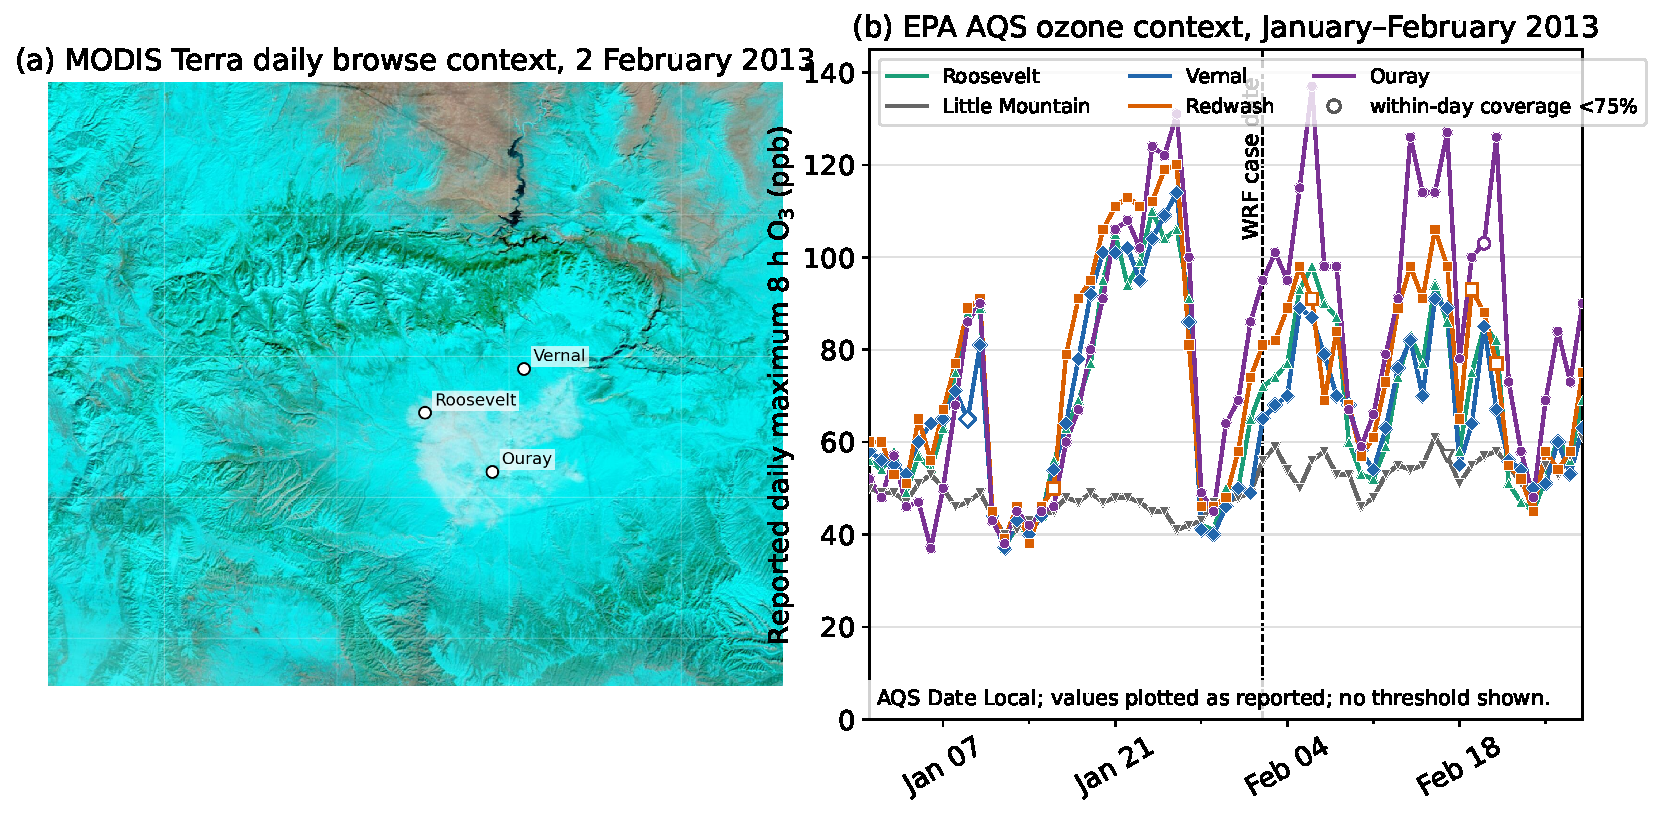
\includegraphics[width=\textwidth]{figures/episode_context_snow_ozone_janfeb2013.pdf}
\caption{Observed context for the 2 February 2013 simulation date.
(a) NASA GIBS Terra MODIS corrected reflectance, bands 7-2-1, for the 2 February calendar day; snow and ice generally appear cyan, most liquid cloud appears white, and ice cloud may also appear cyan.
The browse layer is not a raw-granule crop or quantitative snow retrieval; the nearest centre-covering Terra granule was acquired at 1815--1820 UTC.
(b) EPA AQS first maximum value from the ``Ozone 8-hour 2015'' daily-summary row at Ouray, Redwash, Roosevelt, Vernal, and Little Mountain, converted from ppm to ppb and plotted by AQS local date without recomputation.
All five sites have 59 daily rows; hollow markers identify the seven site-days with less than 75\% within-day observation coverage.
No regulatory threshold is shown, and the panel is episode context rather than chemistry evaluation or meteorology--ozone attribution.}
\label{fig:v3-episode-context}
\end{figure}

\subsection{Observed Surface-Temperature Context}
\label{sec:v3-observed-context}

The basin-floor station repeatedly separated from the higher sites between 31 January and 3 February, while the magnitude and ordering of station temperatures evolved through the diurnal cycle (Figure~\ref{fig:v3-observed}).
The recurring floor-to-bench separation is consistent with a cold-pool surface pattern.
Because the stations are horizontally separated, however, the time series do not determine the cold-pool top, depth, volume, or vertical temperature structure.

\begin{figure}[H]
\centering
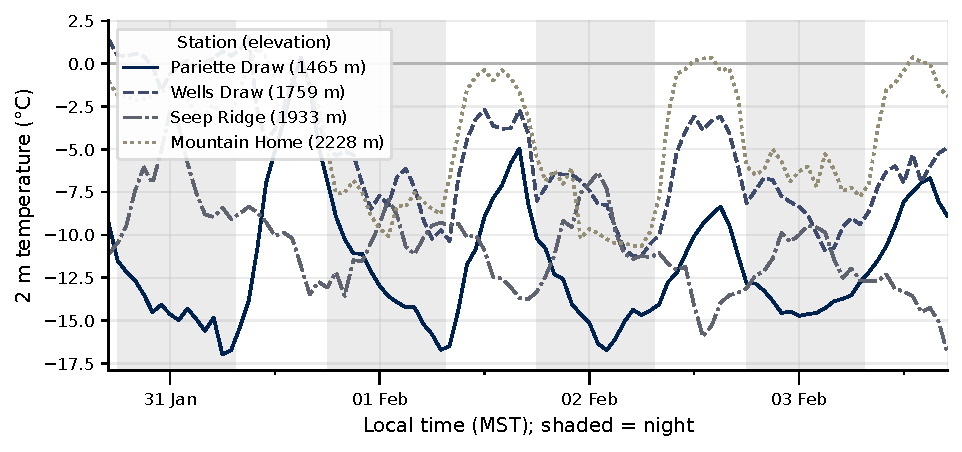
\includegraphics[width=\textwidth]{figures/obs_temp_timeseries_feb0102.pdf}
\caption{Observed 2 m-temperature evolution at four elevation-spanning Uinta Basin stations from 31 January through 3 February 2013.
Shading indicates approximate local night.
The basin-floor site repeatedly separates from the higher sites, and the ordering evolves through the diurnal cycle.
The sites establish a recurring spatial surface-temperature pattern but do not constitute a closely colocated vertical profile.}
\label{fig:v3-observed}
\end{figure}

\subsection{Common-Pipeline Contrasts at a Glance}
\label{sec:v3-effects-panel}

Figure~\ref{fig:v3-effects} compares every controlled contrast evaluated through the common station and common-AGL pipeline.
The two driving-product contrasts are farthest from zero for temperature, fixed-layer stability, and transport wind.
The PBL/surface-layer treatment is smaller, while slope radiation, nest feedback, and the driving-product-by-feedback interaction cluster near zero on those same scales.
Pressure and wind-error metrics follow different orderings, so the panel is a response hierarchy rather than an overall configuration ranking.

\begin{figure}[H]
\centering
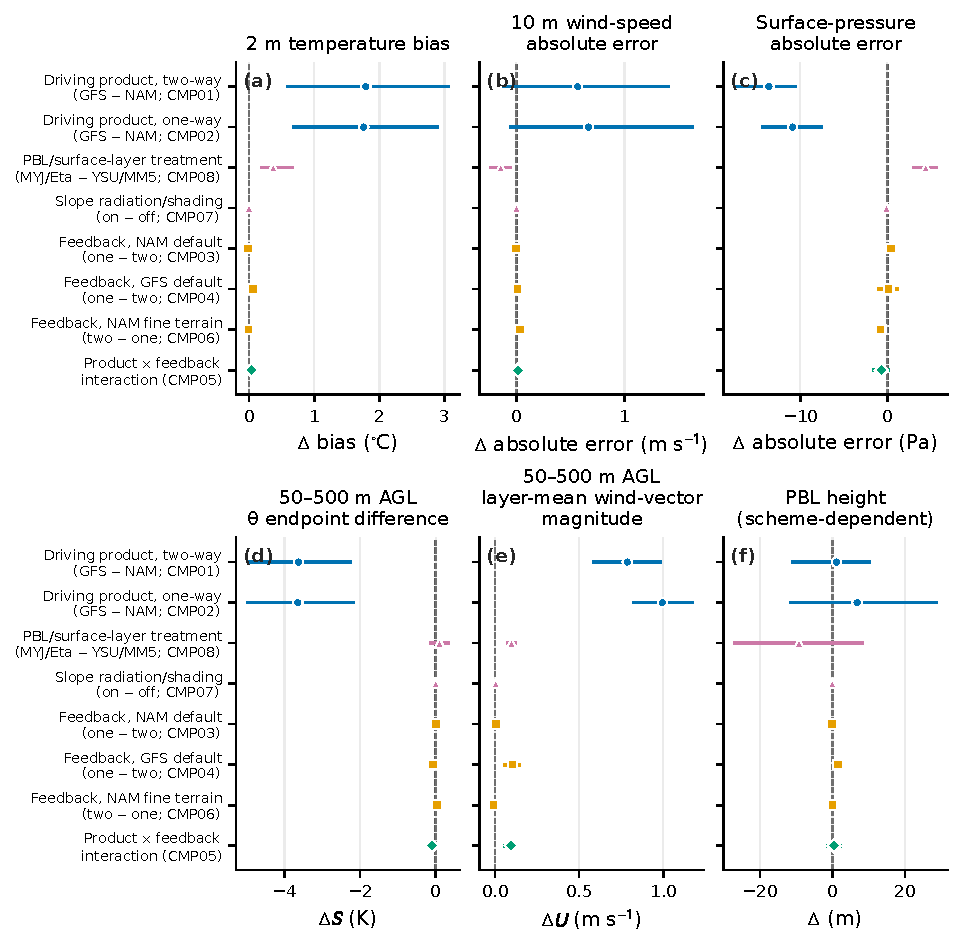
\includegraphics[width=\textwidth]{figures/fig_common_pipeline_effects.pdf}
\caption{Mean five-hour effects for the controlled comparisons that share the station/common-AGL pipeline.
Colours and marker shapes identify driving-product, process-treatment, feedback, and interaction contrasts; each row states its differencing direction.
Driving-product effects are farthest from zero for temperature, fixed-layer stability, and transport wind; the PBL/surface-layer response is smaller, while slope-radiation and feedback effects cluster near zero on those scales.
The different ordering of pressure and wind error prevents interpreting the panel as an overall configuration ranking.
Whiskers are descriptive block-sensitivity intervals for five dependent hourly medians, not confidence intervals.
All values come from the registered common station and common-AGL summaries.}
\label{fig:v3-effects}
\end{figure}

\subsection{Driving-Product Response in the Common Lower Layer}
\label{sec:v3-driving-response}

The two-by-two matrix in Figure~\ref{fig:v3-retention} separates the GFS-versus-NAM driving-product response under one-way and two-way feedback.
Relative to GFS, NAM was 3.63\,K more stable with two-way feedback and 3.65\,K more stable with one-way feedback through the 50--500\,m layer (Table~\ref{tab:v3-effects}).
The five-hour means of hourly spatial-median stability were 7.50 and 7.38\,K for the two GFS runs, compared with 10.82\,K for both NAM members.
The hourly GFS-minus-NAM differences ranged from $-5.58$ to $-1.13$\,K with two-way feedback and from $-5.36$ to $-0.90$\,K with one-way feedback.
All ten product-by-hour stability contrasts therefore retained the same sign.
GFS also increased fixed-layer transport wind by 0.79\,m\,s$^{-1}$ with two-way feedback and 0.99\,m\,s$^{-1}$ with one-way feedback.
The corresponding five-hour means of hourly spatial-median transport wind were approximately 2.0\,m\,s$^{-1}$ for both GFS members and approximately 1.1\,m\,s$^{-1}$ for both NAM members.
The hourly differences ranged from 0.37 to 1.18\,m\,s$^{-1}$ with two-way feedback and from 0.61 to 1.50\,m\,s$^{-1}$ with one-way feedback, with the same sign in every hour.
Native PBL-height differences changed sign within both feedback modes and did not reproduce the stability and wind separation.
This divergence is consistent with the scheme dependence of native PBL-height diagnosis discussed by \citet{Tran2018-ax}.

\begin{figure}[H]
\centering
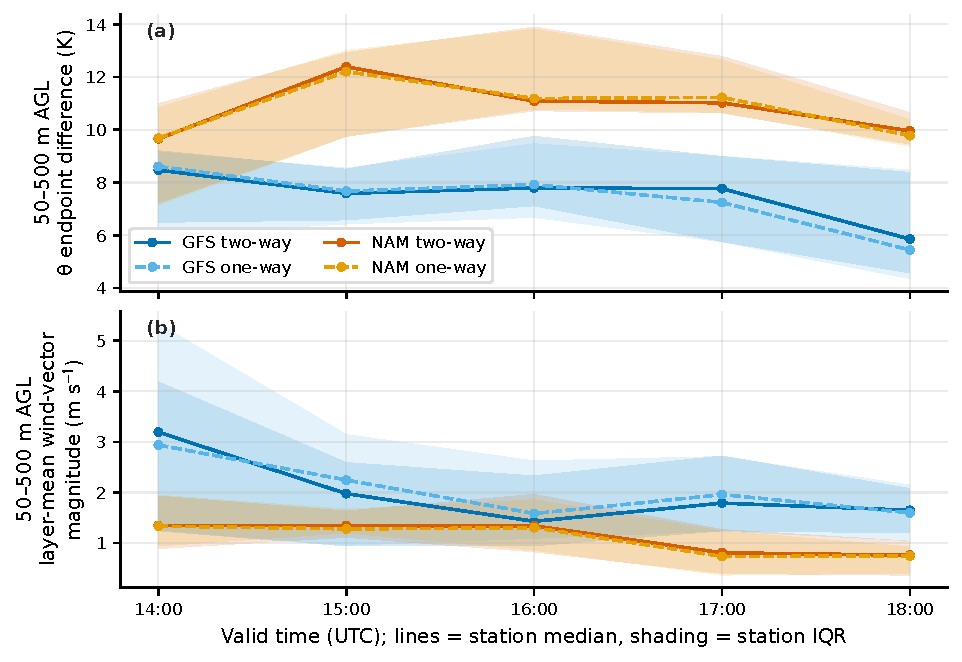
\includegraphics[width=0.82\textwidth]{figures/wrf_retention_ventilation_d02_14to18.pdf}
\caption{Station-column medians and interquartile ranges for 50--500 m AGL potential-temperature stability and fixed-layer transport wind over the matched window.
Solid lines denote two-way feedback and dashed lines denote one-way feedback.
The lower-layer GFS--NAM separation recurs under both feedback modes: GFS is about 3.6 K less stable and 0.8--1.0 m s$^{-1}$ faster in transport wind over the five-hour summary.}
\label{fig:v3-retention}
\end{figure}

\subsection{Surface and Spatial Corroboration}
\label{sec:v3-surface}

The surface-temperature contrasts had the same product ordering as the common-layer diagnostics.
GFS-minus-NAM 2\,m temperature-bias contrasts were +1.79\,$^{\circ}$C with two-way feedback and +1.76\,$^{\circ}$C with one-way feedback (Table~\ref{tab:v3-surface-summary}).
Surface-pressure absolute-error contrasts changed in the opposite direction, at $-13.6$ and $-10.9$\,Pa, while hourly wind absolute-error differences changed sign.
No single surface score therefore provides a general product ranking.
Figure~\ref{fig:v3-bulk-theta} gives a separate two-site surface-structure comparison for the observations and two-way anchor simulations.

\begin{figure}[H]
\centering
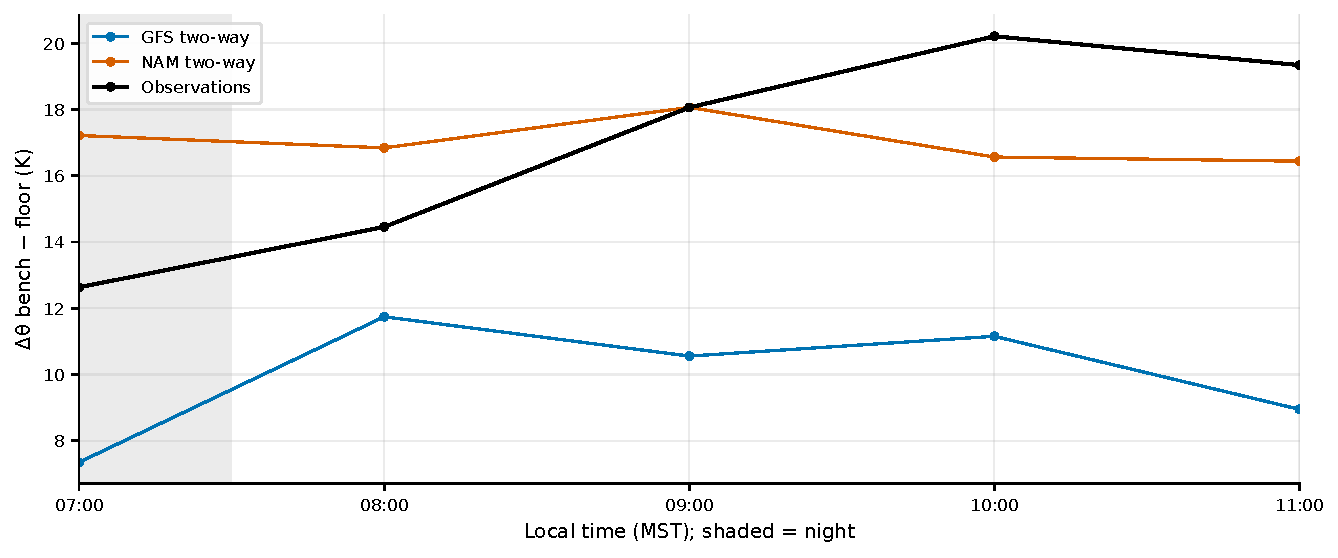
\includegraphics[width=0.82\textwidth]{figures/wrf_inversion_index_feb0102_gfs2way_vs_nam2way_d02_14to18.pdf}
\caption{Observed and modelled Mountain Home-minus-Pariette Draw surface potential-temperature contrast from 1400 to 1800 UTC on 2 February 2013.
The modelled series are X6 (GFS two-way) and X5 (NAM two-way) sampled on d02, and all three series contain the same five retained hourly values after the first two forecast hours were excluded.
The quantity is a horizontally separated bench-minus-floor surface contrast, not inversion depth, a colocated vertical stability measure, or a cold-pool classification threshold.}
\label{fig:v3-bulk-theta}
\end{figure}

The five-hour mean surface potential-temperature contrast between Mountain Home and Pariette Draw was 16.94\,K in the observations, 17.03\,K in NAM two-way, and 9.95\,K in GFS two-way.
The close NAM value corroborates only this horizontally separated surface index; it does not validate modelled inversion depth, vertical structure, or overall surface skill.
Across the registered footprint, the mean GFS-minus-NAM near-surface response was positive and the vertical response remained concentrated below 500 m AGL under both feedback modes (Table~\ref{tab:v3-surface-summary}).
The predeclared spatial-coherence test nevertheless failed because only 64--67\% of footprint cells had the expected sign at 1400--1500 UTC, below the required two-thirds share at every retained hour.
The result is therefore shallow and mean-coherent, but not spatially uniform throughout the retained window.
Later hours were more coherent, but changing an every-hour rule after inspecting those maps would be post hoc.
The maps remain useful descriptive diagnostics without converting the failed test into a passed one.

\subsection{Footprint Heat Deficit: A Weaker State without Faster Loss}
\label{sec:v3-heatdeficit}

The GFS runs retained less footprint-mean, vertically integrated heat deficit at every retained hour under all seven definitions (Section~\ref{sec:v3-heatdeficit-methods}; Table~\ref{tab:v3-heatdeficit}).
Mean GFS-minus-NAM differences were $-1.23$\,MJ\,m$^{-2}$ with two-way feedback and $-1.25$\,MJ\,m$^{-2}$ with one-way feedback.
Primary-definition five-hour means were approximately 3.0\,MJ\,m$^{-2}$ for both GFS runs and approximately 4.2\,MJ\,m$^{-2}$ for both NAM runs.
Every run gained heat deficit from 1400 to 1800 UTC, so the weaker GFS state did not result from demonstrated faster heat-deficit loss during the retained window.
Figure~\ref{fig:v3-heatdeficit-traj} shows the four increasing trajectories and the persistent separation between the two GFS and two NAM members.

\begin{figure}[H]
\centering
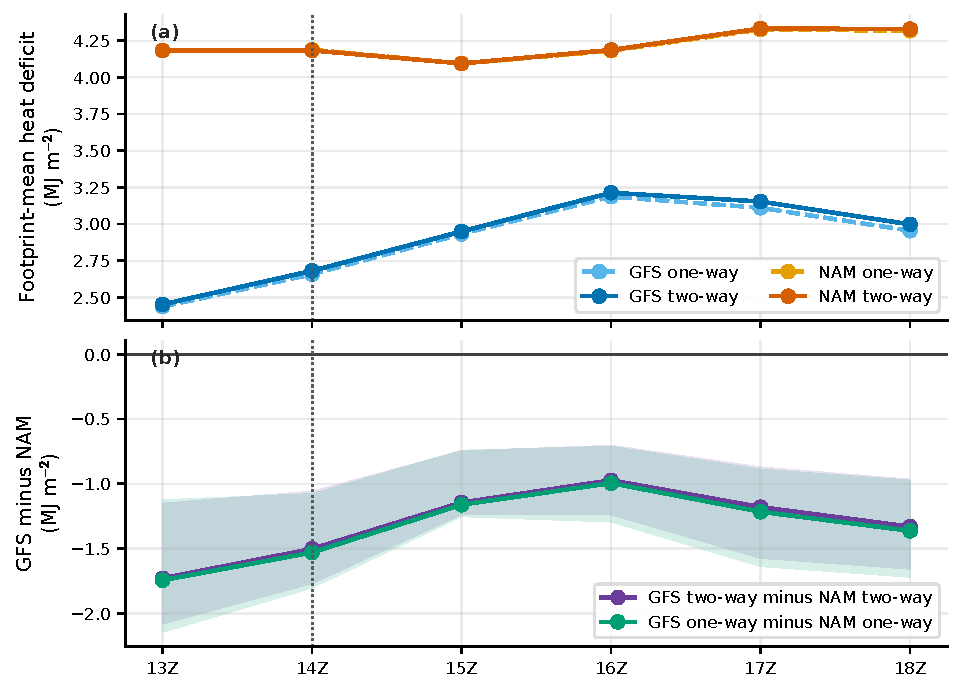
\includegraphics[width=0.82\textwidth]{figures/wrf_heat_deficit_d02_13to18.pdf}
\caption{Footprint-mean heat-deficit trajectories for the four default-terrain matrix members and seven-definition sensitivity envelopes for the two GFS-minus-NAM pairs.
The 1300 UTC values orient the trajectories but are excluded from every reported criterion and effect.
GFS retains a smaller deficit throughout, but the deficit does not decline faster in either GFS member.}
\label{fig:v3-heatdeficit-traj}
\end{figure}

\subsection{Process Treatments on the Fine-Terrain Branch}
\label{sec:v3-process}

The MYJ/Eta versus YSU/revised-MM5 scheme pair changes only the PBL and surface-layer schemes while holding the fine terrain and slope-aware-radiation configuration fixed.
MYJ/Eta increased 2\,m-temperature bias by 0.37\,$^{\circ}$C, reduced 10\,m-wind absolute error by 0.145\,m\,s$^{-1}$, and increased fixed-layer transport wind by 0.098\,m\,s$^{-1}$, with the same sign in all five hours (Supplementary Table~S1).
These changes are smaller than the driving-product response on the shared lower-layer metrics.
The opposing temperature- and wind-error changes do not support an overall scheme-skill ranking.

The slope-radiation addition produced negligible response at the basin-floor station columns.
A spatially organised skin-temperature response appeared on the sidewalls, but the archived flat-plane shortwave field and missing surface heat fluxes could not test the mechanism directly.
The diagnostic is retained in Supplementary Figure~S1 and does not show that slope-aware radiation improved or degraded the cold pool.

\subsection{Nest-Feedback Robustness across Two Terrain Regimes}
\label{sec:v3-feedback}

\label{sec:v3-cmp06}
Within-product feedback effects were small for both GFS and NAM on the default-terrain branch.
The fine-terrain NAM pair reproduced that character: two-way minus one-way feedback increased stability by 0.04\,K and reduced transport wind by 0.01\,m\,s$^{-1}$.
The descriptive block-sensitivity intervals defined in Section~\ref{sec:v3-aggregation} spanned zero for both metrics.
The consistently signed 10\,m-wind and surface-pressure changes were also small and do not support a feedback recommendation beyond this five-hour case.

\subsection{Terrain-Source Brackets}
\label{sec:v3-terrain}

The terrain-source branch holds NAM forcing, one-way feedback, WRF grid spacing, and the YSU/MM5 physics configuration fixed while changing only the static-terrain source.
The three brackets are default minus fine, default minus coarse, and fine minus coarse.
The default-minus-fine response was small on d02 and failed its predeclared terrain-response test.
The wider coarse brackets produced larger spatial responses, but the summary changes with domain support and diagnostic (Supplementary Table~S2).
The controlled fine-minus-coarse composite in Figure~\ref{fig:v3-terrain-cmp11-supplement} therefore shows a reproducible model response without establishing a preferred terrain source, drainage pathway, upstream reservoir, or basin cold-air-volume change.

\begin{figure}[H]
\centering
\IfFileExists{verification/figures/candidates/wrf_terrain_cmp11_d02_d03_16z.pdf}{%
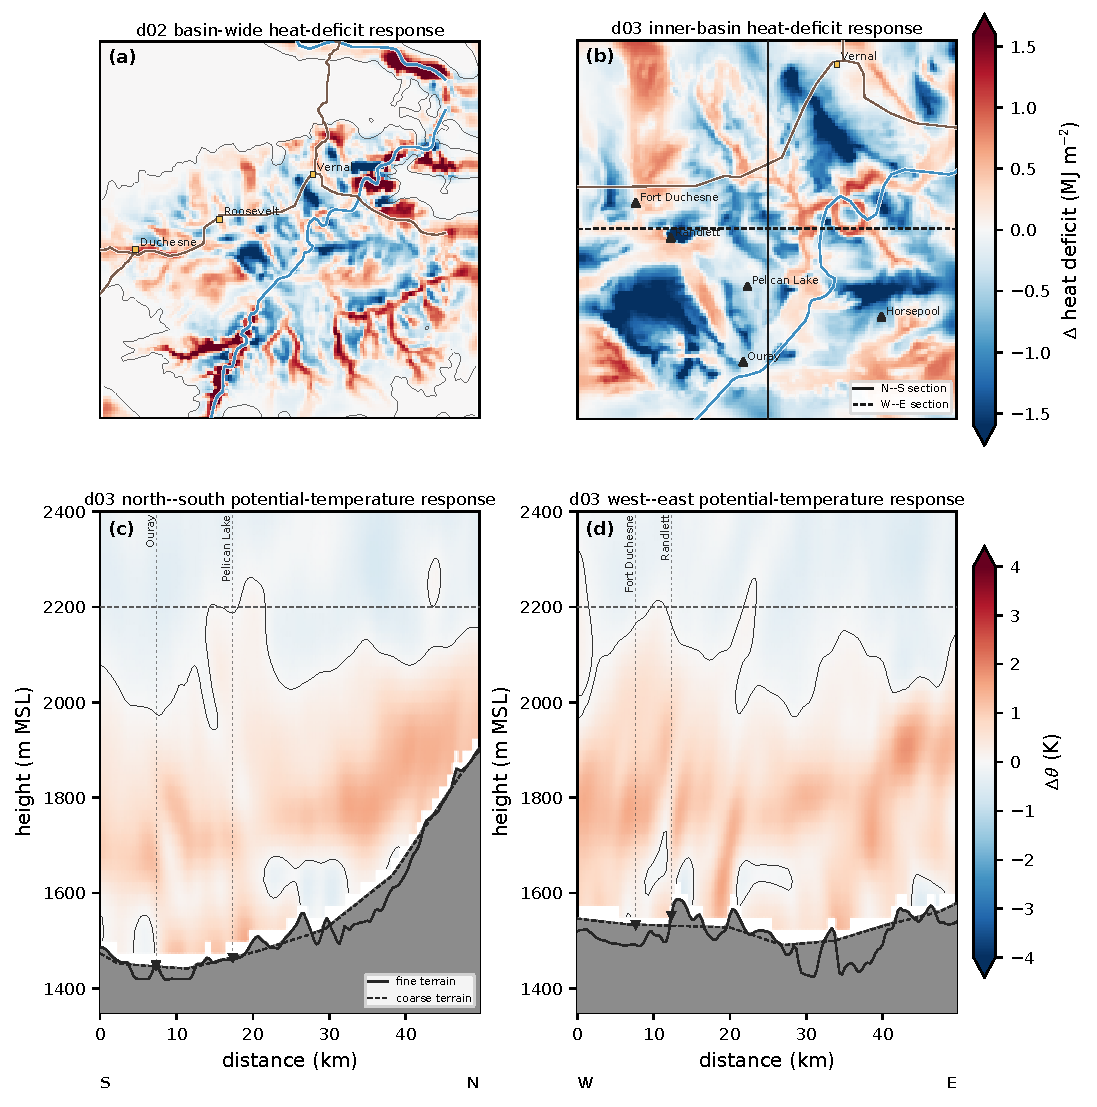
\includegraphics[width=0.96\textwidth]{verification/figures/candidates/wrf_terrain_cmp11_d02_d03_16z.pdf}%
}{\fbox{\parbox[c][0.52\textheight][c]{0.90\textwidth}{\centering Fine-minus-coarse terrain composite unavailable: d02 and d03 top-down heat-deficit maps and orthogonal d03 potential-temperature sections at 1600 UTC.}}}
\caption{Diagnostic response to the widest controlled static-terrain bracket at 1600 UTC, calculated as X0 minus X4 (fine 3-arc-second minus coarse 5-arc-minute source).
(a) The basin-wide d02 and (b) inner-basin d03 top-down heat-deficit maps share a fixed $\pm1.6$ MJ m$^{-2}$ scale.
(c) The north--south and (d) west--east d03 lower-atmosphere potential-temperature sections share a fixed $\pm4$ K scale and the 2200 m crest reference.
The domain-specific panels display spatial and vertical response patterns but rank no terrain source and establish neither drainage direction nor basin cold-air-volume change.}
\label{fig:v3-terrain-cmp11-supplement}
\end{figure}

\section{Discussion}
\label{sec:v3-discussion}

\subsection{The Main Result Is a Difference in the Supplied Lower-Layer State}
\label{sec:v3-disc-supplied-state}

The present study does not seek a universal product or configuration ranking.
Its principal result is a repeated difference in the lower-layer state supplied by the two driving products under both feedback modes.

\begin{itemize}
  \item The GFS-driven runs supplied a warmer, less stable, and faster-moving 50--500\,m layer than feedback-matched NAM members.
  \item The heat-deficit calculation reproduced the same ordering under every registered footprint definition.
  \item Surface pressure and wind error followed different orderings, preventing the response hierarchy from becoming a general skill ranking.
\end{itemize}

The GFS state is more consistent with weaker confinement than the analogous NAM state, but the transport-wind proxy and heat-deficit values are not substitutes for measured mixing volume or basin export.
This distinction matters because errors in confinement, emissions, snow and cloud processes, photolysis, deposition, and chemical mechanism can compensate for one another in coupled simulations \citep{Ahmadov2015-zm,Neemann2015-ws,Matichuk2017-bq}.
A practical future ensemble should therefore vary the treatments that show the largest phenomenon-relevant response, but the present single case cannot prescribe a universal ensemble design.

The model-only d03 Horsepool profiles at 1200 and 1300 UTC (Figure~\ref{fig:v3-spinup-profiles}) expose the source-specific supplied states and their first-hour evolution.
They do not separate early model adjustment from lateral-boundary evolution and do not validate inversion depth.

\begin{figure}[H]
\centering
\begin{minipage}[t]{0.49\textwidth}
\centering
\textbf{(a)}\\[-2pt]
\IfFileExists{figures/theta_profiles_horsepool_gfs_nam_12z.pdf}{%
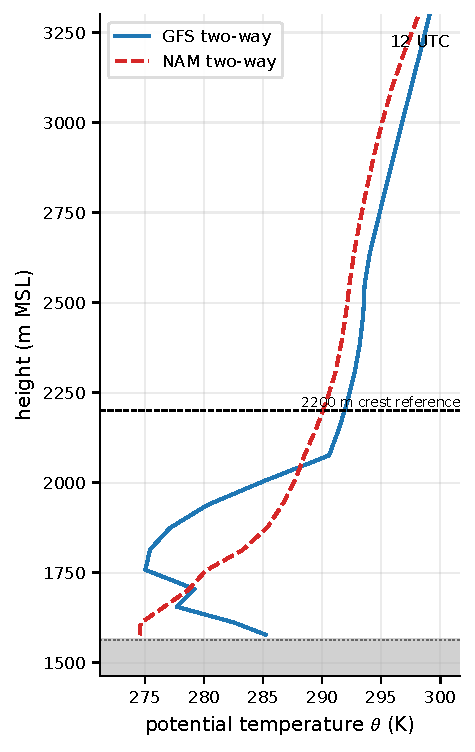
\includegraphics[width=\linewidth]{figures/theta_profiles_horsepool_gfs_nam_12z.pdf}%
}{\fbox{\parbox[c][0.28\textheight][c]{0.88\linewidth}{\centering CHPC render pending: X6 and X5 Horsepool profiles at 1200 UTC.}}}
\end{minipage}\hfill
\begin{minipage}[t]{0.49\textwidth}
\centering
\textbf{(b)}\\[-2pt]
\IfFileExists{figures/theta_profiles_horsepool_gfs_nam_13z.pdf}{%
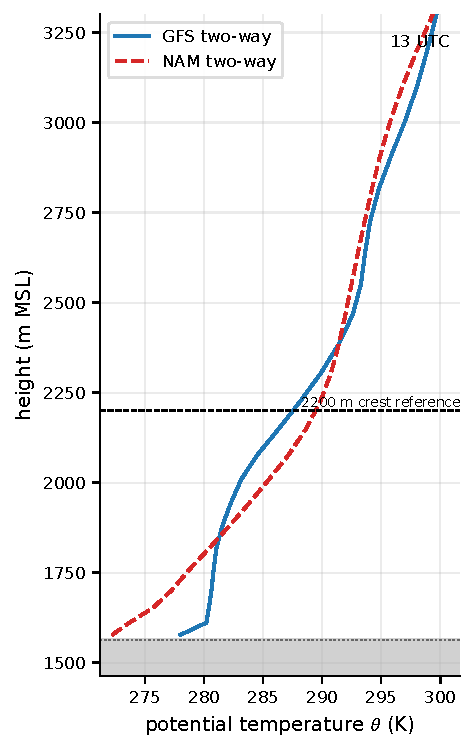
\includegraphics[width=\linewidth]{figures/theta_profiles_horsepool_gfs_nam_13z.pdf}%
}{\fbox{\parbox[c][0.28\textheight][c]{0.88\linewidth}{\centering CHPC render pending: X6 and X5 Horsepool profiles at 1300 UTC.}}}
\end{minipage}
\caption{Model-only d03 potential-temperature profiles at Horsepool for X6 (GFS two-way) and X5 (NAM two-way).
(a) The 1200 UTC initialised states and (b) the 1300 UTC one-hour forecasts use identical axes.
Grey shading marks levels below the local model terrain, and the dashed 2200 m line is the fixed heat-deficit crest reference rather than an observed cold-pool top.
Changes between panels include both early model adjustment and one hour of lateral-boundary evolution; no colocated observed profile validates the modelled layer.}
\label{fig:v3-spinup-profiles}
\end{figure}

\subsection{The Difference Is a State Offset, Not Demonstrated Cold-Pool Loss}
\label{sec:v3-disc-spatial}

The heat-deficit result narrows the interpretation.
GFS had less deficit than NAM under every feedback and footprint definition, but deficit increased in every simulation during the retained window (Figure~\ref{fig:v3-heatdeficit-traj}).
This sheds doubt that it is erosion of the cold pool ("heat-deficit loss") that yields a weaker cold pool after spin-up.
A longer integration through at least one complete diurnal cycle is required to test whether the products differ in cold-pool erosion or persistence.

The spatial analysis gives a similarly bounded result.
The product response was strongest below 500 m AGL and had the expected footprint-mean sign at every hour, but the sign-coherent share fell below two thirds at 1400--1500 UTC.
The response is shallow and mean-coherent on d02, not spatially uniform throughout the window.

\subsection{Secondary Experiments Narrow Rather than Expand the Claim}
\label{sec:v3-disc-process}

The secondary comparisons delimit the driving-product result rather than expanding it into a configuration ranking:

\begin{itemize}
  \item Figure~\ref{fig:v3-effects} shows that the driving-product contrasts are furthest from zero on the common temperature, stability, and transport-wind metrics.
  \item The boundary-layer/surface-layer treatment produced a coherent but smaller response: temperature bias increased while wind absolute error decreased.
  \item Nest-feedback effects remained small on both default- and fine-terrain branches, providing a five-hour robustness check rather than evidence that feedback is generally unimportant.
  \item The slope-radiation response was negligible at the station columns, while the supplementary sidewall diagnostic shows a spatially organised response that the station metric missed.
  \item The controlled terrain brackets show domain- and diagnostic-dependent responses but establish neither a terrain-source ranking nor a drainage or cold-air-volume mechanism.
\end{itemize}

\subsection{Observation and Design Limits Set the Next Experiment}
\label{sec:v3-disc-domains}

These outcomes motivate better measurements and future experiment design, but they do not support radiation or terrain-source superiority claims.
The strongest result is the two-by-two GFS-versus-NAM matrix under one-way and two-way feedback.
Two limitations are especially important for the next experiment:
\begin{itemize}
  \item \textbf{Native PBL height is scheme dependent.} MYJ and YSU need not diagnose the layer top in the same way, so common-height stability and transport remain the more comparable quantities.
  \item \textbf{The floor-to-bench temperature contrast is not vertical validation.} Independent profiles are required to evaluate inversion depth, layer stability, and modelled heat deficit.
\end{itemize}

\section{Conclusions}
\label{sec:v3-conclusions}

The largest repeated response in the controlled archive is the GFS-versus-NAM driving-product contrast on the common d02 evaluation sample.
Relative to NAM, GFS is warmer at the evaluated surface sites, about 3.6 K less stable from 50 to 500 m AGL, 0.8--1.0 m s$^{-1}$ faster in fixed-layer transport wind, and lower in footprint-mean, vertically integrated heat deficit under both feedback modes.
The heat-deficit separation is a state offset, not demonstrated faster loss, and the surface metrics do not support a universal product ranking.
Nest-feedback effects are much smaller, the PBL/surface-layer response is smaller and metric dependent, and the slope-radiation and fine-terrain responses do not support configuration-superiority claims.
The next experiment requires a longer matched matrix, independent vertical observations, a common-support d02--d03 transfer test, and a design that separates initial from lateral-boundary forcing.
The present result does not identify the responsible product component, validate inversion depth, establish event-scale persistence, calculate basin export, or predict ozone.
Within those bounds, the driving-product treatment produced the largest repeated separation in the lower-basin meteorological state supplied to downstream chemistry during the five-hour window.
The numerical summaries supporting the concise Results narrative are retained in Appendix~\ref{app:v3-data}; Supplementary Tables~S1--S2 and Figure~S1 retain the bounded secondary comparisons, terrain summary, and slope-aware-radiation response.

\appendixtitles{yes}
\appendixstart
\appendix
\section{Data Tables and Secondary Diagnostics}
\label{app:v3-data}

This appendix retains the core numerical detail supporting the concise Results narrative.

\begin{table}[H]
\caption{Paired effects for the default-terrain driving-product/feedback matrix, averaged over the five hourly spatial medians.
Positive temperature values indicate a warmer model-minus-observation bias, positive stability values indicate a more stable fixed layer, and positive transport-wind values indicate a larger layer-mean wind.
The effects are deterministic descriptive contrasts rather than inferential estimates.}
\label{tab:v3-effects}
\centering
\begin{tabular}{lrrr}
\toprule
Effect & $\Delta$T2 bias ($^{\circ}$C) & $\Delta S_{50:500}$ (K) & $\Delta U_{50:500}$ (m s$^{-1}$) \\
\midrule
GFS $-$ NAM, two-way & +1.79 & -3.63 & +0.79 \\
GFS $-$ NAM, one-way & +1.76 & -3.65 & +0.99 \\
GFS one-way $-$ two-way & +0.07 & -0.07 & +0.10 \\
NAM one-way $-$ two-way & -0.01 & +0.00 & +0.01 \\
Feedback interaction & +0.04 & -0.10 & +0.10 \\
\bottomrule
\end{tabular}
\end{table}

\begin{table}[H]
\caption{Surface, spatial, and vertical corroboration for the two GFS-minus-NAM driving-product contrasts.
Every value uses the matched station and hour samples described in Section~\ref{sec:v3-surface}.}
\label{tab:v3-surface-summary}
\centering
\small
\begin{tabularx}{\textwidth}{lLL}
\toprule
Diagnostic & Result & Scope \\
\midrule
2 m temperature & GFS-minus-NAM bias contrast +1.79~$^{\circ}$C two-way and +1.76~$^{\circ}$C one-way; absolute-error differences +1.41 and +1.50~$^{\circ}$C & Same ordering as common-AGL stability \\
10 m wind & Bias contrast +0.91 and +0.96 m s$^{-1}$; hourly absolute-error differences change sign & No stable wind-skill ordering \\
Surface pressure & Absolute-error contrast -13.6 Pa two-way and -10.9 Pa one-way; negative in every hour & Opposite ordering from temperature, with small absolute differences \\
Two-site surface index & Observed 12.63--20.21 K; NAM 16.44--18.07 K; GFS 7.35--11.74 K under two-way feedback & Horizontally separated surface contrast, not inversion strength or depth \\
Mean 2 m potential-temperature difference & +0.89 to +1.16 K at 1400--1500 UTC; +2.00 to +2.74 K at 1600--1800 UTC & Positive at all ten pair-hours \\
Footprint sign share & 0.64--0.67 at 1400--1500 UTC; 0.84--0.93 later & Early response is not spatially uniform \\
Low-to-aloft absolute-response ratio & 1.45--3.12 & Response concentrated in the lower atmosphere \\
50--500 m stability difference & -4.33 to -3.04 K & Negative at all ten pair-hours \\
\bottomrule
\end{tabularx}
\end{table}

\begin{table}[H]
\caption{Footprint-mean, vertically integrated heat-deficit contrasts over the 1400--1800 UTC decision window.
The primary definition uses the combined station-and-waypoint hull with a 2200 m crest (4965 cells, 5277 km$^{2}$); envelopes span all seven footprint definitions.
The values are deterministic descriptive contrasts in MJ m$^{-2}$.}
\label{tab:v3-heatdeficit}
\centering
\begin{tabular}{lrr}
\toprule
GFS $-$ NAM quantity & Two-way pair & One-way pair \\
\midrule
Mean difference (primary) & -1.23 & -1.25 \\
Hourly range (primary) & -1.50 to -0.97 & -1.53 to -0.99 \\
Hourly envelope (seven definitions) & -1.77 to -0.70 & -1.80 to -0.71 \\
GFS change, 1400--1800 UTC & +0.32 & +0.30 \\
NAM change, 1400--1800 UTC & +0.15 & +0.13 \\
Difference in change (primary) & +0.17 & +0.17 \\
\bottomrule
\end{tabular}
\end{table}

\vspace{6pt}

\authorcontributions{\textbf{[Author input required: assign and approve CRediT roles for all authors.]}}
\funding{\textbf{[Author input required: insert verified funders and grant numbers.]}}
\institutionalreview{Not applicable.}
\informedconsent{Not applicable.}
\dataavailability{The analysis scripts, derived hourly and paired summaries, heat-deficit tables, selected EPA AQS daily records, run and comparison inventories, provenance records, and promoted figures used for this draft are retained in the private working repository.
Raw WRF inputs and Synoptic observations remain subject to the respective providers' access and reuse terms.}
\acknowledgments{We acknowledge the University of Utah Center for High Performance Computing for computational resources.
We acknowledge Synoptic Data PBC for access to Mesonet API observations.
We thank Brian K. Blaylock for the Herbie and SynopticPy packages, which supported source-data retrieval and Synoptic API access, respectively.\footnote{Herbie: \url{https://doi.org/10.5281/zenodo.4567540}; SynopticPy: \url{https://doi.org/10.5281/zenodo.4567546}.}}
\conflictsofinterest{\textbf{[Author input required: all authors must confirm the conflicts-of-interest statement.]}}
\useofartificialintelligence{Generative artificial intelligence tools, including Anthropic Claude and OpenAI Codex, were used during manuscript preparation to assist with literature synthesis, provenance and analysis-code review, and drafting and editing.
The authors reviewed and edited the resulting material and take responsibility for the content.}

\begin{adjustwidth}{-\extralength}{0cm}
\reftitle{References}
\bibliography{paperpile}
\PublishersNote{}
\end{adjustwidth}

\end{document}
